\documentclass[fleqn, a4paper]{report}

%% Language and font and usefull packages
\usepackage[english]{babel}
\usepackage[utf8x]{inputenc}
\usepackage{booktabs}
\usepackage{tabu}
\usepackage[T1]{fontenc}
\usepackage{bm}
\usepackage{dsfont}
\usepackage{setspace}
\usepackage{amsmath}
\usepackage{graphicx}
\usepackage{fontawesome}
\usepackage{titlepic}
\usepackage{fixltx2e}
\usepackage{booktabs} % For prettier tables
\usepackage[colorinlistoftodos]{todonotes}
\usepackage[colorlinks=true, allcolors=blue]{hyperref}
\usepackage[a4paper,top=1.5cm,bottom=2cm,left=1cm,right=1cm,marginparwidth=1.75cm]{geometry}

\title{Assignment 1 - Generalized Regression Model}

\author{Theodoros Ladas - s2124289
\footnote{University of Edinburgh s2124289@ed.ac.uk}
}
\titlepic{
\includegraphics[width=12.528cm,height=3cm]{./images/edinburgh.png}} 
\date{\parbox{\linewidth}{\centering%
  February 20, 2021\endgraf\bigskip
  Coordinator: Bruce Worton\endgraf\medskip
  Dept.\ of Mathematics \endgraf
  University of Edinburgh}}


\onehalfspacing
\begin{document}
\maketitle

\section*{1. The problem}

The problem in question is to estimate the percentage yield of petroleum spirit from crude oil. The sample for this analysis consists of $n=32$ observations of $4$ explanatory varaibles $x_1,...,x_4$ and one final target variable $y$. 
\begin{itemize}
\item $x_1$: specific gravity of the crude, a function of the API measurment
\item $x_2$: crude oil vapour pressure 
\item $x_3$: the ASTM 10 per cent distilation temperature
\item $x_4$: the petroleum fraction end point
\item   $y$: percentage of petroleum yielded from crude oil
\end{itemize}

The analysis consists of a data-preprocessing and exploration process as well as a comparison of two different but similar linear models in order to find the underlying equation between those $5$ variables. 


\section*{2. The analysis}

We began by exploring the density plots of variables. First of all, we plotted the Kernel Density estimation with a Gaussian Kernel and a bandwidth hyperparameter of the default in \textsf{R}. Figure 1 is the KDE for the target variable $y$, while Figure 2 shows the same for the $X$, where $X$ is the matrix that consists of the vectors of $x_1,\dots,x_4$ as columns, as well as a column of ones, used later for the linear regression model. 

\subsection*{2.1 Data exploration and preprocessing}
\begin{figure}[!h]
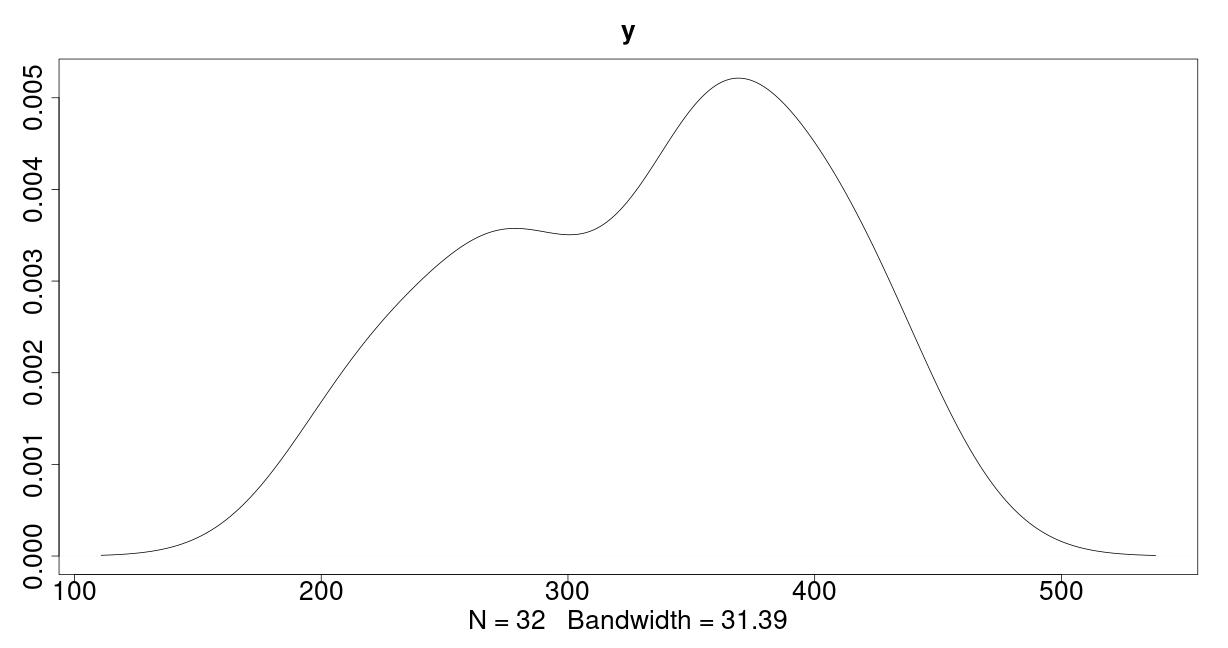
\includegraphics[width=0.35\textwidth]{./images/y_kernel.jpg}
\textsubscript{\textit{Figure 1}}
\label{tab:fig_1}
\end{figure}

\begin{figure}[!h]
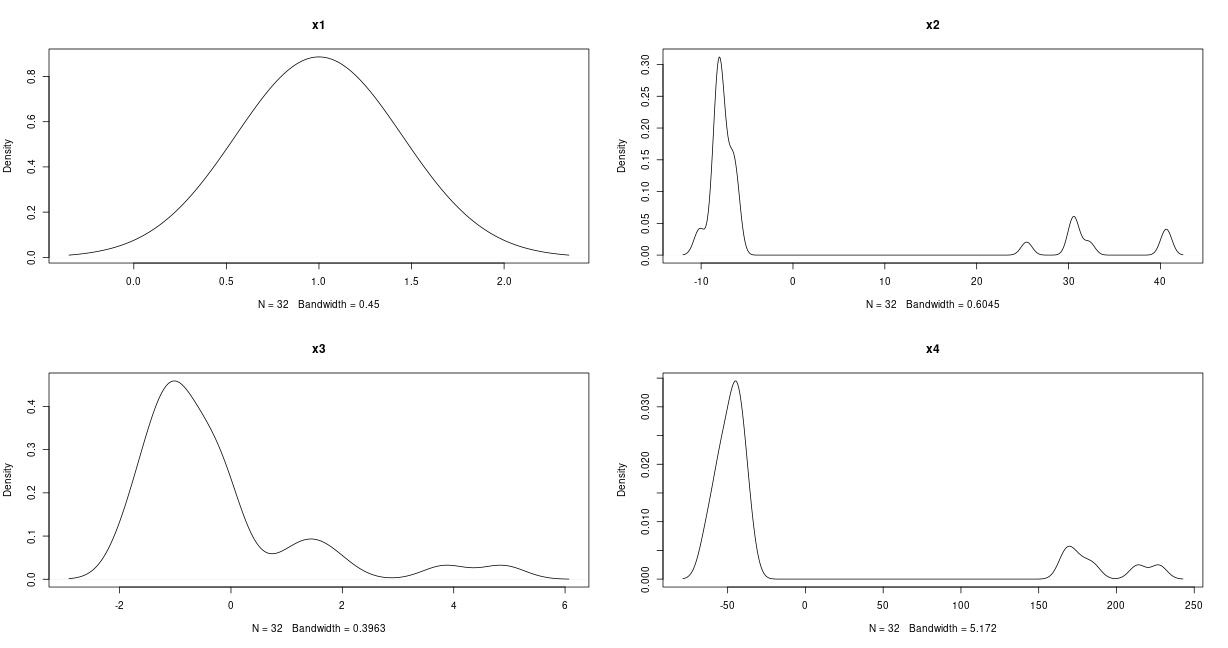
\includegraphics[width=0.35\textwidth]{./images/KDEs.jpg}
\textsubscript{\textit{Figure 2}}
\label{tab:fig_1}
\end{figure}

We can clearly see from that diagram that $x_2,x_3,x_4$ have some structure on their distributions, and specifically $x_3$ has a very similar distribution with the target variable so we suspect that it might be an important variable in our model. The variable $x_1$ on the other hand seems to be normally distributed with $\mu = 1$, which could act as random noise in the model. However, we need to do further tests in order to confirm this. 

Since we only have a small dataset of $n=32$ and four explanatory variables, a linear regression model would be suitable for our analysis. We also considered a Tree-based approach, but this would be better suited for \textit{prediction} instead of finding an expression for the percentage of petroleum yielded from crude oil because the trees do not normally produce coefficients.

Figure 3, shows a heatmap of correlations between the five variables, $x_1,\dots,x_4,y$. This is an important step in the exploration of the data since a linear regression model will be considered for the analysis. We need to check the assumptions of the Ordinary Least Squares method in order to ensure that the coefficients produced will be BLUE (Best Linear Unbiased Estimators). 

\begin{figure}[!h]
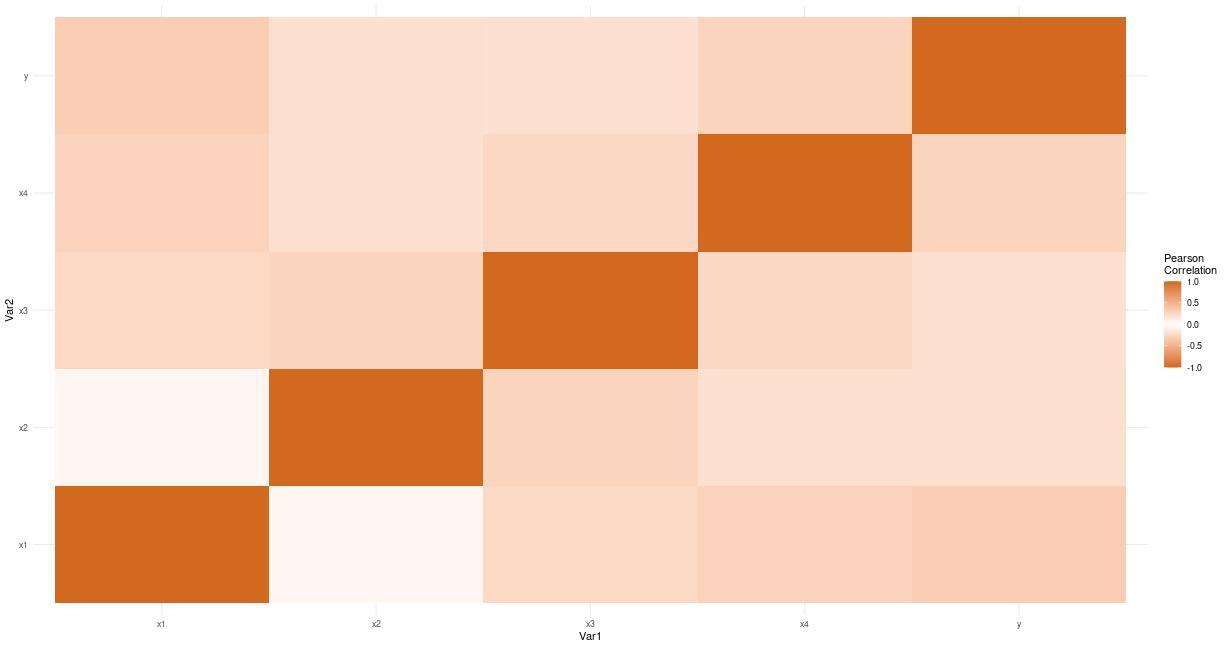
\includegraphics[width=0.35\textwidth]{./images/heatmap.jpg}
\textsubscript{\textit{Figure 3}}
\label{tab:fig_1}
\end{figure}

From the above diagram, we can see that no strong linear correlation between the independent variables is present, therefore no perfect multicollinearity exists in our data. The Pearson Correlation Index is used in this example, with the following formula.

\begin{align*}
r = \frac{\sum(x_i - \bar{x})(s_i - \bar{s})}{\sqrt{\sum(x_i - \bar{x})^2\sum(s_i - \bar{s})^2}}, \text{where}, x \text{~and~} s \text{~columns of the matrix~} X.
\end{align*}


\subsection*{2.2 Models and Results}

\begin{flushleft}
\underline{\large Ridge Regression:} First a Ridge regression model was considered in order to assess whether all the variables we have are important or not. This a technique that shrinks the coefficients of the independent variables, making some of them equal to $0$ \cite{varian2014big}. This has been considered because as we have seen from the KDE estimations of the independent variables, $x_1$ might not be important. The formula for calculating the weights of the ridge regression was \cite{murray_machine_2020}:
\begin{align*}
\beta = (X^TX + \lambda I)^{-1}X^Ty \text{~where the~} \beta \text{~vector, is the vector of the coefficients, and~} \lambda \text{~the hyperparameter.~}
\end{align*}

More details about how the $\lambda$ hyperparameter has been optimized need to be mentioned at this point. A large set of values has been chosen for $\lambda$ from $10^{-20}$ until $10^{10}$, with a step of $0.1$ on the exponent. Then in each iteration, the $\beta$ vector was calculated producing the Mean Square Error. The value for lambda that minimized the MSE was chosen as the best. The values for the weights produced by this algorithm was $\beta = [-6.821,  0.227,  0.554, -0.150,  0.155]$.

\underline{\large Linear Regression:} The linear regression model was build using the default \textsf{glm} package of \textsf{R}. The results produced are identical to the Ridge Regression with insignificant differences in the MSE. Therefore the final model chosen according to the MSE error, is:

$\hat{y} = -6.821 + 0.227 x_1 + 0.554 x_2 -0.150 x_3 + 0.155 x_4$
\end{flushleft}

Other variances of the linear regression model have been considered, where some independent variables have been excluded completely, but all these models yielded worse results, so are not presented here. 

\section*{3. Discussion}

For further analysis, nonlinear (in $X$) models should be considered in order to check whether nonlinearity could yield better results. Also, other types of algorithms such as Bayesian Trees. All the code for the above experiment can be found on my \href{https://github.com/TedOiler/GRM}{\faGithub} page (\url{https://github.com/TedOiler/GRM}). This repository is a private one, that I will make public after the assignment deadline and turn private again when the assignment is graded.

\bibliographystyle{plain}
\bibliography{ref.bib}

\end{document}